% Created by tikzDevice version 0.10.1 on 2017-09-05 19:41:43
% !TEX encoding = UTF-8 Unicode
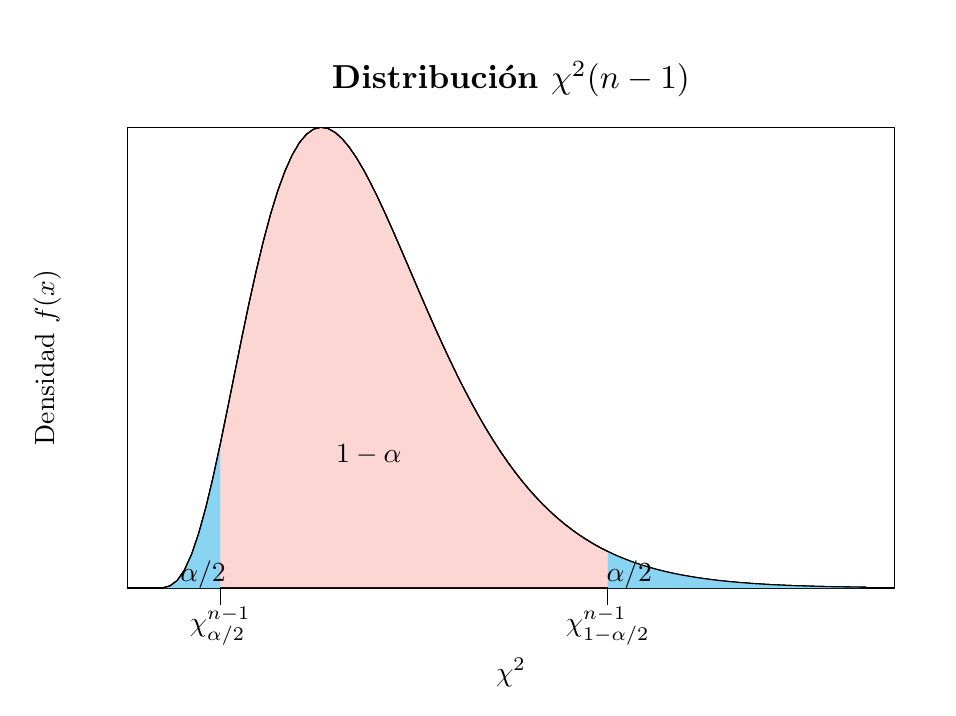
\begin{tikzpicture}[x=1pt,y=1pt]
\definecolor{fillColor}{RGB}{255,255,255}
\path[use as bounding box,fill=fillColor,fill opacity=0.00] (0,0) rectangle (325.21,238.49);
\begin{scope}
\path[clip] ( 36.00, 36.00) rectangle (313.21,202.49);
\definecolor{drawColor}{RGB}{0,0,0}

\path[draw=drawColor,line width= 0.4pt,line join=round,line cap=round] ( 46.27, 36.00) --
	( 48.86, 36.08) --
	( 51.45, 36.78) --
	( 54.05, 38.76) --
	( 56.64, 42.50) --
	( 59.23, 48.19) --
	( 61.82, 55.84) --
	( 64.42, 65.24) --
	( 67.01, 76.10) --
	( 69.60, 88.05) --
	( 72.19,100.68) --
	( 74.79,113.60) --
	( 77.38,126.43) --
	( 79.97,138.84) --
	( 82.57,150.55) --
	( 85.16,161.34) --
	( 87.75,171.01) --
	( 90.34,179.46) --
	( 92.94,186.59) --
	( 95.53,192.38) --
	( 98.12,196.83) --
	(100.71,199.95) --
	(103.31,201.82) --
	(105.90,202.49) --
	(108.49,202.07) --
	(111.09,200.64) --
	(113.68,198.31) --
	(116.27,195.19) --
	(118.86,191.38) --
	(121.46,186.98) --
	(124.05,182.10) --
	(126.64,176.83) --
	(129.23,171.25) --
	(131.83,165.46) --
	(134.42,159.51) --
	(137.01,153.48) --
	(139.61,147.42) --
	(142.20,141.39) --
	(144.79,135.44) --
	(147.38,129.59) --
	(149.98,123.89) --
	(152.57,118.35) --
	(155.16,113.00) --
	(157.75,107.85) --
	(160.35,102.92) --
	(162.94, 98.22) --
	(165.53, 93.75) --
	(168.13, 89.51) --
	(170.72, 85.50) --
	(173.31, 81.73) --
	(175.90, 78.18) --
	(178.50, 74.85) --
	(181.09, 71.73) --
	(183.68, 68.83) --
	(186.27, 66.12) --
	(188.87, 63.60) --
	(191.46, 61.27) --
	(194.05, 59.10) --
	(196.65, 57.10) --
	(199.24, 55.25) --
	(201.83, 53.55) --
	(204.42, 51.98) --
	(207.02, 50.54) --
	(209.61, 49.21) --
	(212.20, 48.00) --
	(214.79, 46.89) --
	(217.39, 45.87) --
	(219.98, 44.94) --
	(222.57, 44.09) --
	(225.17, 43.32) --
	(227.76, 42.61) --
	(230.35, 41.97) --
	(232.94, 41.39) --
	(235.54, 40.86) --
	(238.13, 40.38) --
	(240.72, 39.95) --
	(243.31, 39.55) --
	(245.91, 39.20) --
	(248.50, 38.87) --
	(251.09, 38.58) --
	(253.69, 38.32) --
	(256.28, 38.08) --
	(258.87, 37.87) --
	(261.46, 37.67) --
	(264.06, 37.50) --
	(266.65, 37.34) --
	(269.24, 37.20) --
	(271.83, 37.08) --
	(274.43, 36.96) --
	(277.02, 36.86) --
	(279.61, 36.77) --
	(282.21, 36.69) --
	(284.80, 36.61) --
	(287.39, 36.55) --
	(289.98, 36.49) --
	(292.58, 36.44) --
	(295.17, 36.39) --
	(297.76, 36.35) --
	(300.36, 36.31) --
	(302.95, 36.27);
\end{scope}
\begin{scope}
\path[clip] (  0.00,  0.00) rectangle (325.21,238.49);
\definecolor{drawColor}{RGB}{0,0,0}

\path[draw=drawColor,line width= 0.4pt,line join=round,line cap=round] ( 36.00, 36.00) --
	(313.21, 36.00) --
	(313.21,202.49) --
	( 36.00,202.49) --
	( 36.00, 36.00);
\end{scope}
\begin{scope}
\path[clip] (  0.00,  0.00) rectangle (325.21,238.49);
\definecolor{drawColor}{RGB}{0,0,0}

\node[text=drawColor,anchor=base,inner sep=0pt, outer sep=0pt, scale=  1.20] at (174.61,216.35) {\bfseries Distribución $\chi^2(n-1)$};

\node[text=drawColor,anchor=base,inner sep=0pt, outer sep=0pt, scale=  1.00] at (174.61,  2.40) {$\chi^2$};

\node[text=drawColor,rotate= 90.00,anchor=base,inner sep=0pt, outer sep=0pt, scale=  1.00] at (  9.60,119.25) {Densidad $f(x)$};
\end{scope}
\begin{scope}
\path[clip] ( 36.00, 36.00) rectangle (313.21,202.49);
\definecolor{fillColor}{RGB}{137,211,243}

\path[fill=fillColor] ( 46.27, 36.00) --
	( 46.27, 36.00) --
	( 48.86, 36.08) --
	( 51.45, 36.78) --
	( 54.05, 38.76) --
	( 56.64, 42.50) --
	( 59.23, 48.19) --
	( 61.82, 55.84) --
	( 64.42, 65.24) --
	( 67.01, 76.10) --
	( 69.60, 88.05) --
	( 69.60, 36.00) --
	cycle;
\definecolor{drawColor}{RGB}{0,0,0}

\path[draw=drawColor,line width= 0.4pt,line join=round,line cap=round] ( 46.27, 36.00) --
	( 48.86, 36.08) --
	( 51.45, 36.78) --
	( 54.05, 38.76) --
	( 56.64, 42.50) --
	( 59.23, 48.19) --
	( 61.82, 55.84) --
	( 64.42, 65.24) --
	( 67.01, 76.10) --
	( 69.60, 88.05) --
	( 72.19,100.68) --
	( 74.79,113.60) --
	( 77.38,126.43) --
	( 79.97,138.84) --
	( 82.57,150.55) --
	( 85.16,161.34) --
	( 87.75,171.01) --
	( 90.34,179.46) --
	( 92.94,186.59) --
	( 95.53,192.38) --
	( 98.12,196.83) --
	(100.71,199.95) --
	(103.31,201.82) --
	(105.90,202.49) --
	(108.49,202.07) --
	(111.09,200.64) --
	(113.68,198.31) --
	(116.27,195.19) --
	(118.86,191.38) --
	(121.46,186.98) --
	(124.05,182.10) --
	(126.64,176.83) --
	(129.23,171.25) --
	(131.83,165.46) --
	(134.42,159.51) --
	(137.01,153.48) --
	(139.61,147.42) --
	(142.20,141.39) --
	(144.79,135.44) --
	(147.38,129.59) --
	(149.98,123.89) --
	(152.57,118.35) --
	(155.16,113.00) --
	(157.75,107.85) --
	(160.35,102.92) --
	(162.94, 98.22) --
	(165.53, 93.75) --
	(168.13, 89.51) --
	(170.72, 85.50) --
	(173.31, 81.73) --
	(175.90, 78.18) --
	(178.50, 74.85) --
	(181.09, 71.73) --
	(183.68, 68.83) --
	(186.27, 66.12) --
	(188.87, 63.60) --
	(191.46, 61.27) --
	(194.05, 59.10) --
	(196.65, 57.10) --
	(199.24, 55.25) --
	(201.83, 53.55) --
	(204.42, 51.98) --
	(207.02, 50.54) --
	(209.61, 49.21) --
	(212.20, 48.00) --
	(214.79, 46.89) --
	(217.39, 45.87) --
	(219.98, 44.94) --
	(222.57, 44.09) --
	(225.17, 43.32) --
	(227.76, 42.61) --
	(230.35, 41.97) --
	(232.94, 41.39) --
	(235.54, 40.86) --
	(238.13, 40.38) --
	(240.72, 39.95) --
	(243.31, 39.55) --
	(245.91, 39.20) --
	(248.50, 38.87) --
	(251.09, 38.58) --
	(253.69, 38.32) --
	(256.28, 38.08) --
	(258.87, 37.87) --
	(261.46, 37.67) --
	(264.06, 37.50) --
	(266.65, 37.34) --
	(269.24, 37.20) --
	(271.83, 37.08) --
	(274.43, 36.96) --
	(277.02, 36.86) --
	(279.61, 36.77) --
	(282.21, 36.69) --
	(284.80, 36.61) --
	(287.39, 36.55) --
	(289.98, 36.49) --
	(292.58, 36.44) --
	(295.17, 36.39) --
	(297.76, 36.35) --
	(300.36, 36.31) --
	(302.95, 36.27);

\node[text=drawColor,anchor=base,inner sep=0pt, outer sep=0pt, scale=  1.00] at ( 63.38, 38.30) {$\alpha/2$};
\end{scope}
\begin{scope}
\path[clip] (  0.00,  0.00) rectangle (325.21,238.49);
\definecolor{drawColor}{RGB}{0,0,0}

\path[draw=drawColor,line width= 0.4pt,line join=round,line cap=round] ( 69.60, 36.00) -- ( 69.60, 36.00);

\path[draw=drawColor,line width= 0.4pt,line join=round,line cap=round] ( 69.60, 36.00) -- ( 69.60, 30.00);

\node[text=drawColor,anchor=base,inner sep=0pt, outer sep=0pt, scale=  1.00] at ( 69.60, 20.40) {$\chi_{\alpha/2}^{n-1}$};
\end{scope}
\begin{scope}
\path[clip] ( 36.00, 36.00) rectangle (313.21,202.49);
\definecolor{fillColor}{RGB}{137,211,243}

\path[fill=fillColor] (209.61, 36.00) --
	(209.61, 49.21) --
	(212.20, 48.00) --
	(214.79, 46.89) --
	(217.39, 45.87) --
	(219.98, 44.94) --
	(222.57, 44.09) --
	(225.17, 43.32) --
	(227.76, 42.61) --
	(230.35, 41.97) --
	(232.94, 41.39) --
	(235.54, 40.86) --
	(238.13, 40.38) --
	(240.72, 39.95) --
	(243.31, 39.55) --
	(245.91, 39.20) --
	(248.50, 38.87) --
	(251.09, 38.58) --
	(253.69, 38.32) --
	(256.28, 38.08) --
	(258.87, 37.87) --
	(261.46, 37.67) --
	(264.06, 37.50) --
	(266.65, 37.34) --
	(269.24, 37.20) --
	(271.83, 37.08) --
	(274.43, 36.96) --
	(277.02, 36.86) --
	(279.61, 36.77) --
	(282.21, 36.69) --
	(284.80, 36.61) --
	(287.39, 36.55) --
	(289.98, 36.49) --
	(292.58, 36.44) --
	(295.17, 36.39) --
	(297.76, 36.35) --
	(300.36, 36.31) --
	(302.95, 36.27) --
	(302.95, 36.00) --
	cycle;
\definecolor{fillColor}{RGB}{238,50,36}

\path[fill=fillColor,fill opacity=0.20] ( 69.60, 36.00) --
	( 69.60, 88.05) --
	( 72.19,100.68) --
	( 74.79,113.60) --
	( 77.38,126.43) --
	( 79.97,138.84) --
	( 82.57,150.55) --
	( 85.16,161.34) --
	( 87.75,171.01) --
	( 90.34,179.46) --
	( 92.94,186.59) --
	( 95.53,192.38) --
	( 98.12,196.83) --
	(100.71,199.95) --
	(103.31,201.82) --
	(105.90,202.49) --
	(108.49,202.07) --
	(111.09,200.64) --
	(113.68,198.31) --
	(116.27,195.19) --
	(118.86,191.38) --
	(121.46,186.98) --
	(124.05,182.10) --
	(126.64,176.83) --
	(129.23,171.25) --
	(131.83,165.46) --
	(134.42,159.51) --
	(137.01,153.48) --
	(139.61,147.42) --
	(142.20,141.39) --
	(144.79,135.44) --
	(147.38,129.59) --
	(149.98,123.89) --
	(152.57,118.35) --
	(155.16,113.00) --
	(157.75,107.85) --
	(160.35,102.92) --
	(162.94, 98.22) --
	(165.53, 93.75) --
	(168.13, 89.51) --
	(170.72, 85.50) --
	(173.31, 81.73) --
	(175.90, 78.18) --
	(178.50, 74.85) --
	(181.09, 71.73) --
	(183.68, 68.83) --
	(186.27, 66.12) --
	(188.87, 63.60) --
	(191.46, 61.27) --
	(194.05, 59.10) --
	(196.65, 57.10) --
	(199.24, 55.25) --
	(201.83, 53.55) --
	(204.42, 51.98) --
	(207.02, 50.54) --
	(209.61, 49.21) --
	(209.61, 36.00) --
	cycle;
\definecolor{drawColor}{RGB}{0,0,0}

\path[draw=drawColor,line width= 0.4pt,line join=round,line cap=round] ( 46.27, 36.00) --
	( 48.86, 36.08) --
	( 51.45, 36.78) --
	( 54.05, 38.76) --
	( 56.64, 42.50) --
	( 59.23, 48.19) --
	( 61.82, 55.84) --
	( 64.42, 65.24) --
	( 67.01, 76.10) --
	( 69.60, 88.05) --
	( 72.19,100.68) --
	( 74.79,113.60) --
	( 77.38,126.43) --
	( 79.97,138.84) --
	( 82.57,150.55) --
	( 85.16,161.34) --
	( 87.75,171.01) --
	( 90.34,179.46) --
	( 92.94,186.59) --
	( 95.53,192.38) --
	( 98.12,196.83) --
	(100.71,199.95) --
	(103.31,201.82) --
	(105.90,202.49) --
	(108.49,202.07) --
	(111.09,200.64) --
	(113.68,198.31) --
	(116.27,195.19) --
	(118.86,191.38) --
	(121.46,186.98) --
	(124.05,182.10) --
	(126.64,176.83) --
	(129.23,171.25) --
	(131.83,165.46) --
	(134.42,159.51) --
	(137.01,153.48) --
	(139.61,147.42) --
	(142.20,141.39) --
	(144.79,135.44) --
	(147.38,129.59) --
	(149.98,123.89) --
	(152.57,118.35) --
	(155.16,113.00) --
	(157.75,107.85) --
	(160.35,102.92) --
	(162.94, 98.22) --
	(165.53, 93.75) --
	(168.13, 89.51) --
	(170.72, 85.50) --
	(173.31, 81.73) --
	(175.90, 78.18) --
	(178.50, 74.85) --
	(181.09, 71.73) --
	(183.68, 68.83) --
	(186.27, 66.12) --
	(188.87, 63.60) --
	(191.46, 61.27) --
	(194.05, 59.10) --
	(196.65, 57.10) --
	(199.24, 55.25) --
	(201.83, 53.55) --
	(204.42, 51.98) --
	(207.02, 50.54) --
	(209.61, 49.21) --
	(212.20, 48.00) --
	(214.79, 46.89) --
	(217.39, 45.87) --
	(219.98, 44.94) --
	(222.57, 44.09) --
	(225.17, 43.32) --
	(227.76, 42.61) --
	(230.35, 41.97) --
	(232.94, 41.39) --
	(235.54, 40.86) --
	(238.13, 40.38) --
	(240.72, 39.95) --
	(243.31, 39.55) --
	(245.91, 39.20) --
	(248.50, 38.87) --
	(251.09, 38.58) --
	(253.69, 38.32) --
	(256.28, 38.08) --
	(258.87, 37.87) --
	(261.46, 37.67) --
	(264.06, 37.50) --
	(266.65, 37.34) --
	(269.24, 37.20) --
	(271.83, 37.08) --
	(274.43, 36.96) --
	(277.02, 36.86) --
	(279.61, 36.77) --
	(282.21, 36.69) --
	(284.80, 36.61) --
	(287.39, 36.55) --
	(289.98, 36.49) --
	(292.58, 36.44) --
	(295.17, 36.39) --
	(297.76, 36.35) --
	(300.36, 36.31) --
	(302.95, 36.27);

\node[text=drawColor,anchor=base,inner sep=0pt, outer sep=0pt, scale=  1.00] at (217.39, 38.30) {$\alpha/2$};
\end{scope}
\begin{scope}
\path[clip] (  0.00,  0.00) rectangle (325.21,238.49);
\definecolor{drawColor}{RGB}{0,0,0}

\path[draw=drawColor,line width= 0.4pt,line join=round,line cap=round] (209.61, 36.00) -- (209.61, 36.00);

\path[draw=drawColor,line width= 0.4pt,line join=round,line cap=round] (209.61, 36.00) -- (209.61, 30.00);

\node[text=drawColor,anchor=base,inner sep=0pt, outer sep=0pt, scale=  1.00] at (209.61, 20.40) {$\chi_{1-\alpha/2}^{n-1}$};
\end{scope}
\begin{scope}
\path[clip] ( 36.00, 36.00) rectangle (313.21,202.49);
\definecolor{drawColor}{RGB}{0,0,0}

\node[text=drawColor,anchor=base,inner sep=0pt, outer sep=0pt, scale=  1.00] at (123.27, 81.47) {$1-\alpha$};
\end{scope}
\end{tikzpicture}
